\documentclass{acmsiggraph}
\usepackage[english]{babel}
\usepackage[T1]{fontenc}
\usepackage[latin1]{inputenc}
\usepackage{float, enumitem, footnote, multirow}
\usepackage[font=scriptsize,labelfont=bf, justification=centering, format=hang]{caption}
\usepackage{subfig}
\usepackage{amsmath, amsthm, amssymb, bbm}
\usepackage[ruled,vlined]{algorithm2e}
\usepackage{hyperref}
\usepackage{microtype}
\usepackage{lmodern}
\usepackage{listings}
\lstset{
	basicstyle=\footnotesize
}
\graphicspath{{../figures/}}
\DeclareMathOperator\sign{sign}

\newcommand\mycommfont[1]{\footnotesize\ttfamily{#1}}
\SetCommentSty{mycommfont}
\newcommand{\R}{\mathbb{R}}
\newcommand{\1}{\mathbbm{1}}

\title{Machine Learning for Computer Vision\\ {\large [MVA 2015/2016]}\\
\vspace{10pt}
Programming Assignment 2}

\author{Maha ELBAYAD
%\\ \texttt{maha.elbayad@student.ecp.fr}}
}
\pdfauthor{Maha ELBAYAD}
\newcommand{\E}{\mathbb{E}}
\begin{document}
\maketitle
\section{Support Vector Machine classifiers}
We use LibSVM library to train a C-SVM with rbf kernel. To choose the best couple of parameters $C$ (regularization) and $\gamma$ (rbf kernel parameter $K(x,y)=exp(-\gamma\|x-y\|^2)$) we consider a 10-folds cross-validation.
\begin{figure}[H]
\centering
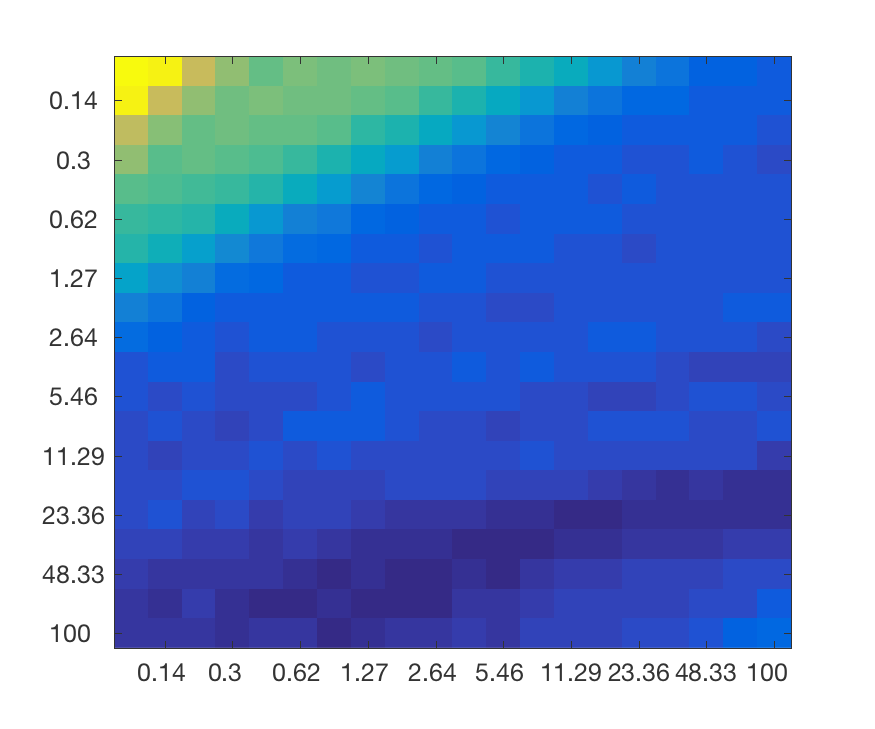
\includegraphics[width=5cm]{cv_error}
\caption*{Best perfromance achieved with $(\gamma,C)=(33.5982,5.4556)$}
\end{figure}
After training on the full set we obtain the boundary decision shown below with the support vectors.
\begin{figure}[H]
\centering
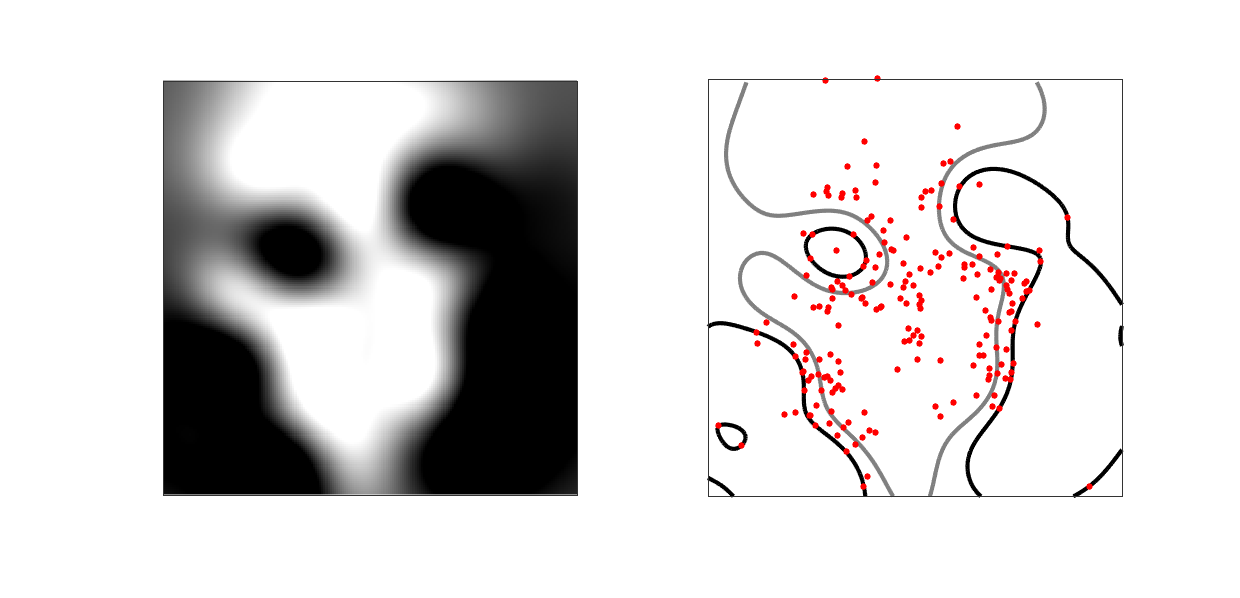
\includegraphics[width=8cm]{values_svm}
\caption*{Decision boundary (svm probabilities on a grid) and support vectors}
\end{figure}
With this model we achieved an error rate of 17.80\% (89/500)

\section{Adaboost}
We implemented the Adaboost algorithm where at each round $t$ we fit a weak learner $h_t(x)$ to the training data $\mathcal X ={(x_n,y_n)_{1\leq n\leq N}}$ by minimizing:
\[L_t = \sum_{n=1}^Nw_n^{(t)}\1[h_t(x_n)\neq y_n]\]
We initialize the weights at $w_i^{(0)} =\frac{1}{N},\:\forall i$ and update at each round as follows:
\[\begin{split}
\epsilon_t  &= \frac{\sum_{n=1}^N w_n^{(t)} \1[h_t(x_n)\neq y_n]}{\sum_{n=1}^Nw_n^{(t)}}\\
\alpha_t & = \log\left(\frac{1 - \epsilon_t}{\epsilon_t}\right)\\
w_n^{(t+1)} &= \frac{1}{Z_t}w_n^{(t)} \exp\left(-\alpha_t h_t(x_n) y_n\right)
\end{split}\]
where $Z_t$ is a scaling factor so that the weights sum to 1.\\
The final strong model makes predictions given by:
\[H_T(x)=\sum_{t=1}^T\alpha_th_t(x)\]
The error of the boosted model is estimated as:
\[E_T = \frac{1}{N}\sum_{n=1}^N \1[sign(H_T(x_n))\neq y_n]\]
We can estimate an upper bound of $E_T$ with:
\[\widetilde E_T = \sum_{n=1}^N\exp\left(-y_nH_T(x_n)\right) = \prod_{t=1}^TZ_t\]
On the right figure we report the error defined as the number of misclassified samples from the training set while on the left one we plot the normalized errors $E_T$ and $\widetilde E_T$.
\begin{figure}[H]
\centering
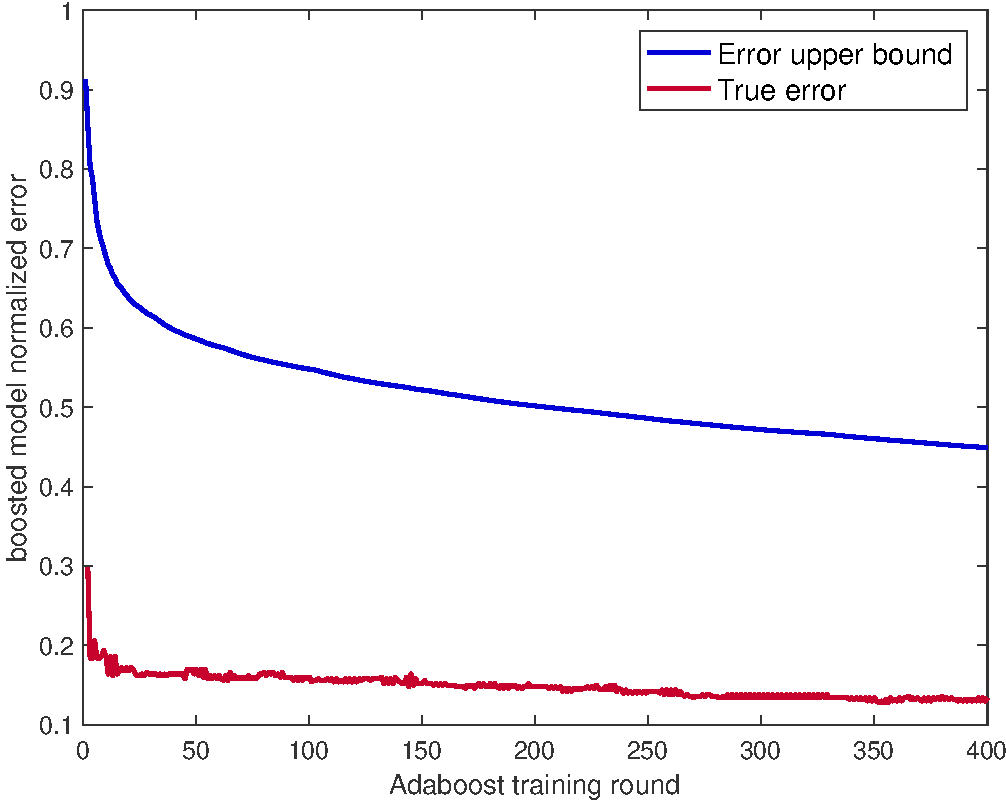
\includegraphics[height=4cm]{loss_adaboost}%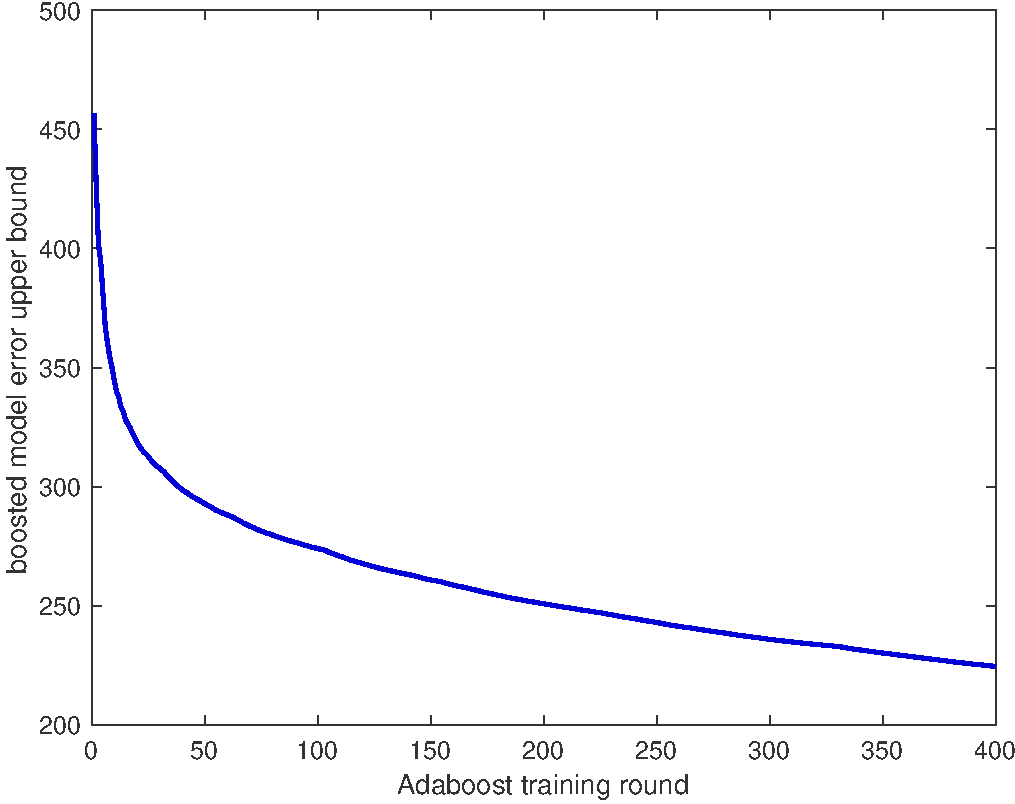
\includegraphics[height=4cm]{loss_adaboost_bound}
\caption*{Error of the strong model $f = \sign H_t$ at each round}
\end{figure}

\begin{figure}[H]
\centering
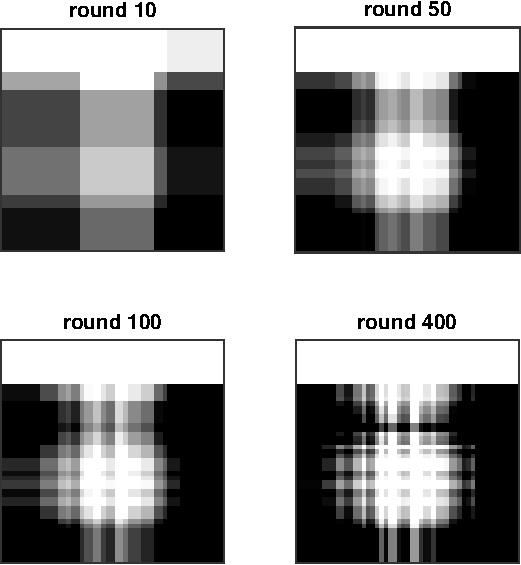
\includegraphics[width=6cm]{per_round}
\caption*{Strong models $H_{10}, H_{50}, H_{100},H_{400}$}
\end{figure}

\begin{figure}[H]
\centering
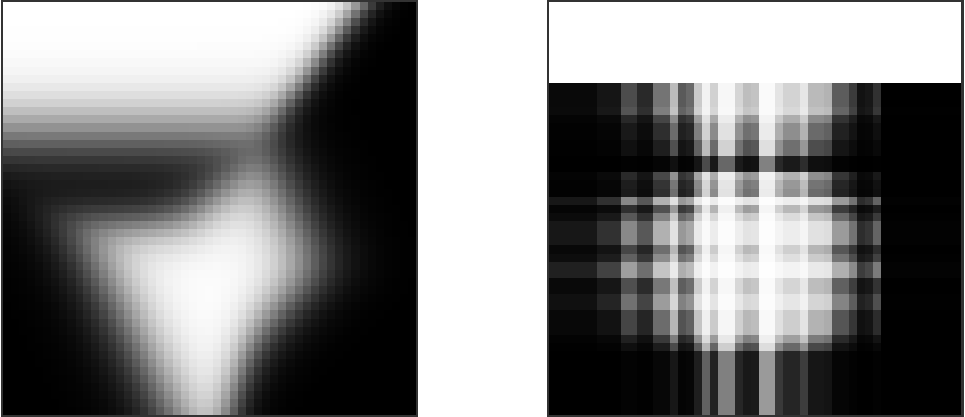
\includegraphics[width=6cm]{classifiers}
\caption*{Left: true class posterior  - Right: Final adaboost classifier }
\end{figure}

\subsection{SVM vs. Adaboost}
We measure the Adaboost performance on the same test set as the SVM above. The decision boundaries are shown below with the test set samples scattered to visualize the quality of each model. The test error rate of the Adaboost classifier is 21.40\% vs 17.80\% for the SVM while on the training set Adaboost misclassified 67/500 and the SVM 69/500. Visually the probability distribution obtained with the SVM is much closer to the ground truth prior. 
\begin{figure}[H]
\centering
\subfloat[Train]{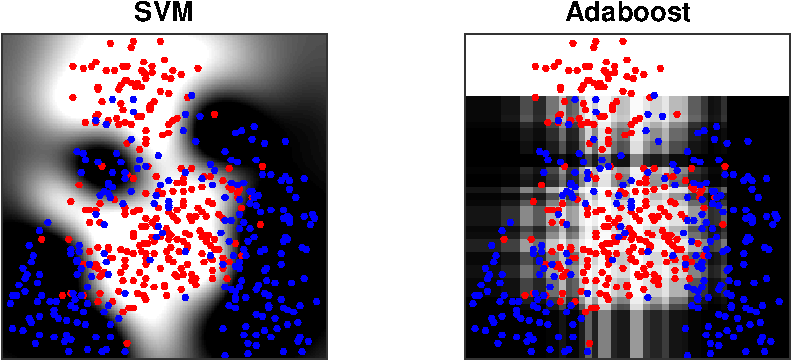
\includegraphics[width=6cm]{db_train}}\\
\subfloat[Test]{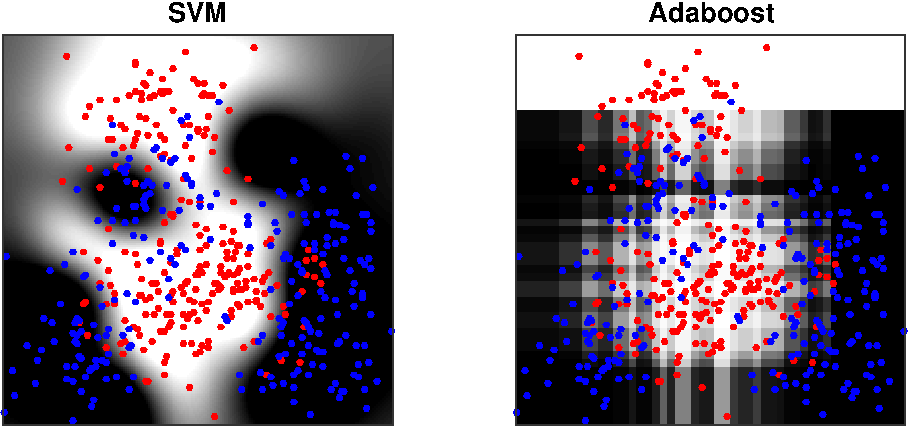
\includegraphics[width=6cm]{db}}
\caption*{SVM vs Adaboost}
\end{figure} 

\end{document}